\documentclass[12pt,a4paper]{article}

\usepackage[margin=1in]{geometry}
\usepackage{graphicx}
\usepackage{setspace}
\usepackage{times}
\usepackage{titlesec}
\usepackage{amsmath, amssymb, amsthm}
\usepackage{booktabs}
\usepackage{array}
\usepackage{hyperref}
\usepackage{enumitem}
\usepackage{fancyhdr}
\setlength{\headheight}{14.5pt}
\usepackage{indentfirst}
\usepackage{xcolor}
\usepackage{tikz}
\usetikzlibrary{positioning, arrows.meta, shapes.geometric, fit, calc}

\newcommand{\fillin}[1]{\textcolor{red}{[#1]}}
\newcommand{\blank}{\textcolor{red}{[\hspace{1cm}]}}
\newcommand{\figplaceholder}[3]{%
  \begin{figure}[h!]
    \centering
    \fbox{\parbox[c][#1][c]{0.9\linewidth}{\centering\textcolor{gray}{[INSERT IMAGE HERE]}}}
    \caption{#2}\label{#3}
  \end{figure}}

\hypersetup{
    colorlinks=true,
    linkcolor=black,
    citecolor=black,
    urlcolor=blue
}

\onehalfspacing
\setlength{\parindent}{0.5in}
\setlength{\parskip}{0pt}

\widowpenalty=10000
\clubpenalty=10000


\newcommand{\cmdline}[1]{\par\nopagebreak\smallskip\noindent\colorbox{black!6}{\,\texttt{#1}\,}\par\smallskip}

\titleformat{\section}
    {\normalfont\bfseries\large}{\thesection.}{0.5em}{}
\titleformat{\subsection}
    {\normalfont\bfseries}{\thesubsection.}{0.5em}{}

\pagestyle{fancy}
\fancyhf{}
\fancyhead[L]{Webcam-Based Third-Person to First-Person Motion Mapping}
\fancyhead[R]{\thepage}
\renewcommand{\headrulewidth}{0.4pt}

\newcommand{\UniversityName}{Bulacan State University}
\newcommand{\CollegeName}{College of Science}
\newcommand{\CourseCode}{MCS 306}
\newcommand{\CourseDescription}{Introduction to Artificial Intelligence}
\newcommand{\AcademicYear}{Academic Year 2026--2027}
\newcommand{\StudyTitle}{Real-Time Webcam-Based Third-Person to First-Person Motion Mapping Using MediaPipe and Confidence-Aware Head-Pose Estimation}
\newcommand{\AuthorNames}{
	Ignacio, Clarence Wayne B.\\
	Florano, Aldred F.\\
	Maniacop, Clive Job V.\\
	Panuncio, David James G.\\
	Santos, Sherwin Aisner N. }
\newcommand{\CourseYearSection}{BS Mathematics 3B}
\newcommand{\InstructorName}{Aarhus M. Dela Cruz}
\newcommand{\SubmissionDate}{11, 02, 2026}

% Logo file paths
\newcommand{\BulSULogo}{assets/bulsu.png}
\newcommand{\COSLogo}{assets/college_of_science.png}

\begin{document}

\begin{titlepage}
    \centering

    \begin{minipage}{0.22\textwidth}
        \centering
        \includegraphics[width=0.95\linewidth]{\BulSULogo}
    \end{minipage}
    \hfill
    \begin{minipage}{0.50\textwidth}
        \centering
        {\Large\bfseries \UniversityName\par}
        \vspace{0.15cm}
        {\large\bfseries \CollegeName\par}
        \vspace{0.15cm}
        {\normalsize \CourseCode: \CourseDescription\par}
        \vspace{0.15cm}
        {\normalsize \AcademicYear\par}
    \end{minipage}
    \hfill
    \begin{minipage}{0.22\textwidth}
        \centering
        \includegraphics[width=0.95\linewidth]{\COSLogo}
    \end{minipage}

    \vspace{1.2in}

    {\Large\bfseries MINI RESEARCH AND EXPOSITION PAPER\par}

    \vspace{0.5in}

    {\LARGE\bfseries \StudyTitle\par}

    \vspace{0.8in}

    {\large\bfseries Authors\par}
    \vspace{0.2cm}
    {\large \AuthorNames\par}

    \vspace{0.5in}

    {\large \CourseYearSection\par}
    \vfill
    {\normalsize Submitted to:\par}
    \vspace{0.15cm}
    {\normalsize\bfseries \InstructorName\par}
    \vspace{0.4in}
    {\normalsize \SubmissionDate\par}
\end{titlepage}
\pagenumbering{roman}
\setcounter{page}{1}


\begin{abstract}
\noindent This paper presents a webcam-based prototype that maps third-person hand landmarks into a first-person coordinate representation. The system uses MediaPipe Pose, Hand, and Face Landmarkers to estimate body, hand, and facial information from webcam frames. A head-relative coordinate frame is established using estimated head position and orientation, and a $4\times4$ homogeneous matrix transformation is used to express wrist and finger landmarks relative to that frame. To reduce instability when the face is partially covered, the prototype applies confidence-aware head-pose estimation by considering landmark visibility and hand occlusion, combining facial and pose-based orientation estimates, and using temporal prediction and adaptive smoothing. The paper explains the mathematical concepts and processing stages behind the prototype, presents its implementation, and identifies tests needed to evaluate detection continuity, view stability, recovery behavior, and processing speed. The output is a geometric representation of mapped hands and fingers rather than a reconstructed photographic first-person scene. Quantitative performance and integration with external game or VR applications remain subjects for further testing.
\end{abstract}

\noindent\textbf{Keywords:} MediaPipe, human pose estimation, first-person motion mapping, matrix transformation, occlusion-robust head tracking

\newpage
\tableofcontents
\newpage

\pagenumbering{arabic}
\setcounter{page}{1}

\section{Introduction}

Virtual reality (VR) and interactive applications use movement as a means of interacting with digital environments. However, capturing human movement may require specialized equipment, increasing the cost and complexity of implementation. Advances in artificial intelligence (AI) and computer vision provide an alternative through webcam-based human pose estimation, which uses machine-learning models to detect body landmarks.

This paper presents a real-time webcam-based 3D motion-mapping system that uses MediaPipe to estimate human body landmarks and a custom coordinate-based matrix algorithm to map third-person movement into a corresponding first-person representation. The study demonstrates the application of AI-based pose estimation and mathematical computation in real-time motion processing, with potential applications in virtual reality, avatar animation, and gesture-based interaction.

\subsection{Objectives of the Paper}

The objectives of this paper are as follows:

\begin{enumerate}[label=\arabic*.]
    \item To introduce the concept of real-time webcam-based 3D motion mapping from a third-person to a first-person representation;
    \item To explain the relevant concepts of AI-based human pose estimation, 3D coordinate systems, and matrix transformations used in the proposed system;
    \item  To demonstrate the application of MediaPipe and a custom matrix-transformation algorithm in mapping human body movements in real time; and
    \item To summarize the system's potential applications, capabilities, and limitations in first-person interaction, virtual reality, and avatar animation.
\end{enumerate}

\section{Review of Related Literature and Background Concepts}

This section discusses existing studies and background concepts related to AI-based human pose estimation, 3D motion reconstruction, and motion mapping. These studies provide the theoretical and technical foundation for the proposed webcam-based system, which uses MediaPipe to estimate body landmarks and a custom coordinate-transformation algorithm to map third-person movements into a corresponding first-person motion representation.

\subsection{Key Definitions}
\begin{itemize}
    \item \textbf{Artificial Intelligence (AI).} Artificial Intelligence refers to the development of computer systems capable of performing tasks that typically require human intelligence. In this study, AI is used through MediaPipe's machine-learning-based pose estimation to identify human body landmarks from webcam input.

    \item \textbf{Computer Vision.} Computer vision is a field of AI that enables computers to interpret and process visual information from images and videos. In this study, it enables the system to analyze webcam footage and estimate the positions of human body landmarks.

    \item \textbf{Human Pose Estimation.} Human pose estimation is the process of identifying and estimating the positions of body landmarks, such as the shoulders, elbows, wrists, and hips, from visual input. The proposed system uses MediaPipe to obtain these landmarks as input for subsequent motion processing.

    \item \textbf{MediaPipe.} MediaPipe is a framework that provides tools for building machine-learning and computer-vision applications. In this study, its Pose Landmarker functionality is used to estimate human body landmarks from webcam footage.

    \item \textbf{Three-Dimensional (3D) Coordinates.} Three-dimensional coordinates represent a point's position along three axes, commonly denoted as $x$, $y$, and $z$. The proposed system uses estimated 3D body-landmark coordinates to represent and process human movement in three-dimensional space.

    \item \textbf{Real-Time Processing.} Real-time processing refers to processing incoming data quickly enough to support timely responses as new data arrives. In this study, it refers to processing webcam frames and mapping the detected body movements as the video is captured.

    \item \textbf{Coordinate System.} A coordinate system is a reference framework used to specify the positions of points in space. In this study, coordinate systems provide the basis for representing detected body landmarks and mapping their positions to the intended first-person representation.

    \item \textbf{Matrix Transformation.} A matrix transformation is a mathematical operation that uses a matrix to transform coordinates, such as by rotating, scaling, or changing the orientation of points. In the proposed system, coordinate-based matrix transformations are used to map detected body movements into a corresponding first-person motion representation.

    \item \textbf{Third-Person Perspective.} A third-person perspective refers to a viewpoint in which a person is observed externally, such as through a webcam positioned in front of or beside the person. In this study, it describes the viewpoint from which the system captures the user's movements.

    \item \textbf{First-Person Motion Representation.} A first-person motion representation describes movement mapped into a coordinate arrangement intended to correspond to movement from the user's own perspective. In this study, it is the target representation produced by transforming the estimated third-person body movements.
\end{itemize}


\subsection{Related Studies}
The following studies are relevant to the present research as they provide foundational knowledge on AI-based human pose estimation, real-time 3D pose reconstruction, and motion mapping through coordinate transformations. These studies help establish existing approaches, the technologies and mathematical methods used, and their respective capabilities and limitations. By examining their methodologies and findings, the present study identifies concepts and techniques applicable to the development of a webcam-based system that maps third-person human movements into a corresponding first-person motion representation. The reviewed studies also provide a basis for understanding how the proposed system relates to existing approaches and how its coordinate-transformation method differs from those primarily focused on pose estimation, 3D avatar animation, or robotic motion imitation.

    \subsubsection{AI-Based Human Pose Estimation}
    AI-Based Human Pose Estimation is the use of artificial intelligence to detect human motion and map those motions to its relevant joints or keypoints. It is an integral part of this research, as it provides the capability to interpret body-motions and turn them into usable data. The following paper serves as an exposition regarding its relevance to the study.

        \paragraph{BlazePose: On-device Real-time Body Pose Tracking}
        Bazarevsky et al. (2020) presented BlazePose, a pose-estimation method designed to track human body landmarks in real time. The study is relevant to the present research because it demonstrates how machine-learning models can estimate body landmarks from visual input. This supports the use of AI-based pose estimation as the initial stage of the proposed webcam-based motion-mapping system.
        
        \paragraph{Feasibility of 3D Body Tracking from Monocular 2D Video Feeds in Musculoskeletal Telerehabilitation}
        The study investigates the feasibility of using MediaPipe Pose to estimate three-dimensional human body movements from monocular 2D video footage for physiotherapy applications. The researchers evaluated eight exercises by comparing the estimated joint ranges of motion against ground-truth measurements. The results showed strong correlations for several exercises, while others presented challenges due to occlusion, unusual poses, and depth ambiguity. This study is relevant to the present research because it demonstrates the potential of MediaPipe for markerless 3D human pose estimation using a single camera, while highlighting limitations that may affect the accuracy of estimated body coordinates. These findings provide useful context for the proposed system, which uses MediaPipe-derived landmarks as input for a custom matrix-transformation algorithm to map third-person movements into a corresponding first-person motion representation.

    \subsubsection{Motion Mapping and Spatial Transformation}
    Motion mapping and spatial transformation involve transferring movement data from one coordinate system or spatial representation to another while preserving the intended movement relationships. These techniques are relevant to the present study because they provide the mathematical foundation for transforming body landmarks detected by MediaPipe into a corresponding first-person motion representation. By applying coordinate-based matrix transformations, the proposed system aims to convert third-person webcam-tracked movements into their corresponding mapped positions in real time.

        \paragraph{Retargeting Human-Object Interaction to Virtual Avatars}
        The study by Kim et al. (2016) presents a spatial mapping approach for transferring human-object interactions to virtual avatars while maintaining relevant pose and spatial relationships. This is relevant to the present study because it demonstrates how spatial correspondences can be established to transfer motion between different representations. A similar concept may be investigated for mapping MediaPipe-derived body landmarks to their corresponding positions in a first-person coordinate system. However, the original method focuses on human-object interaction and avatar retargeting, so its suitability for the proposed third-person-to-first-person motion-mapping pipeline must be assessed rather than assumed.

        \paragraph{Enhanced real-time motion transfer to 3D avatars using RGB-based human 3D pose estimation}The study presents a real-time human motion-transfer approach that uses RGB camera input and MediaPipe to estimate 3D body landmarks, correct landmark inaccuracies—particularly in the depth dimension—and transfer the resulting motion to a 3D avatar. By relying on an ordinary RGB camera rather than specialized motion-capture equipment, the approach offers a more accessible method of capturing and reproducing human movement. This study is relevant to the present research because it demonstrates how MediaPipe-derived landmarks can be processed and transformed to produce a different motion representation. Similarly, the proposed system uses MediaPipe to estimate body landmarks and applies a custom coordinate-based matrix transformation to map third-person movements into a corresponding first-person motion representation. However, while the referenced study focuses on animating 3D avatars, the present research focuses on coordinate-based motion mapping rather than avatar animation.

    \subsubsection{Real-Time 3D Human Pose Reconstruction}
    Real-time 3D human pose reconstruction involves estimating a person's body position and movement in three-dimensional space from visual input, such as webcam footage. This is relevant to the present study because the proposed system uses MediaPipe to detect body landmarks and obtain coordinate data for processing. These estimated coordinates serve as the input for the system's custom matrix-transformation algorithm, which maps third-person body movements into a corresponding first-person motion representation in real time.

        \paragraph{Real-time 3D Human Pose and Motion Reconstruction from Monocular RGB Videos}
        Yiannakides et al. (2019) investigated the reconstruction of 3D human pose and motion from monocular video. This work provides related context for estimating three-dimensional human movement using a single monocular camera. It can help establish the background for this study's proposed system, which also uses webcam input to obtain body-motion information.


\section{Methodology or Expository Framework}

This paper follows an expository framework supported by a working Python prototype. The prototype uses MediaPipe's Pose, Hand, and Face Landmarkers to obtain body, hand, and facial data from webcam frames. NumPy is used for coordinate and matrix operations, while OpenCV handles webcam input and visualization. The system maps the detected hands into a first-person representation relative to an estimated head coordinate frame.

\subsection{System Components}

\subsubsection{Landmark Groups Used}

The prototype uses the landmark groups summarized in Table~\ref{tab:landmarks}. Head landmarks establish the position and orientation of the first-person coordinate frame. Wrist landmarks provide the position of each hand, while the Hand Landmarker supplies the detailed finger landmarks.

\begin{table}[h!]
    \centering
    \caption{Landmark groups used by the prototype}
    \label{tab:landmarks}
    \small
    \begin{tabular}{>{\raggedright\arraybackslash}p{2.2cm} >{\raggedright\arraybackslash}p{3.6cm} >{\raggedright\arraybackslash}p{3.4cm} >{\raggedright\arraybackslash}p{4.6cm}}
        \toprule
        Body part & Source model & Landmarks / output & Role in the system \\
        \midrule
        Head & Pose Landmarker; Face Landmarker & Nose, eyes, ears; facial transformation matrix and selected face-mesh points & Estimates the origin and orientation of the first-person frame \\
        Hands & Pose Landmarker; Hand Landmarker & Wrists; 21 landmarks per detected hand & Establishes hand position and finger configuration \\
        \bottomrule
    \end{tabular}
\end{table}

\subsubsection{Coordinate Systems}

The prototype obtains 3D world landmarks from MediaPipe Pose. The coordinates are converted to a right-handed convention with $x$ pointing right, $y$ pointing up, and $z$ pointing toward the camera. This is the third-person coordinate frame used to represent the detected landmarks.

The first-person coordinate frame is attached to the estimated head pose. Its origin is the midpoint between the eyes, and its axes represent right, up, and forward relative to the head. This allows the system to express hand positions relative to the estimated viewpoint rather than relative to the webcam image.


\begin{figure}[h!]
    \centering
    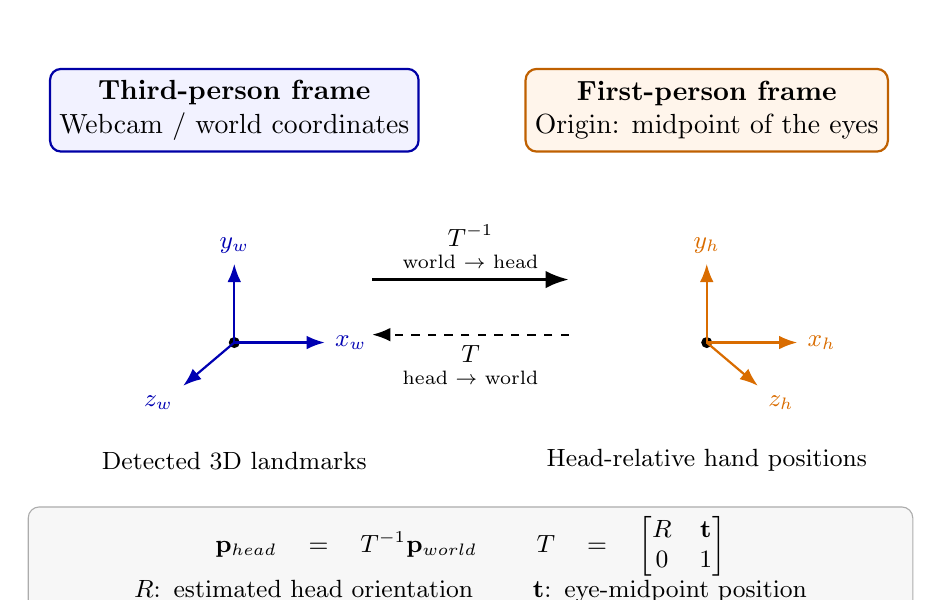
\begin{tikzpicture}[>=Latex, axis/.style={->,thick},
        world/.style={draw=blue!65!black,thick,rounded corners,fill=blue!5,minimum width=3.1cm,minimum height=1.05cm,align=center},
        head/.style={draw=orange!75!black,thick,rounded corners,fill=orange!8,minimum width=3.1cm,minimum height=1.05cm,align=center},
        lab/.style={font=\small}]
        \node[world] at (-3,2.5) {\textbf{Third-person frame}\\Webcam / world coordinates};
        \coordinate (O) at (-3,-0.45);
        \fill (O) circle (2pt);
        \draw[axis,blue!70!black] (O)--++(1.15,0) node[right,lab] {$x_w$};
        \draw[axis,blue!70!black] (O)--++(0,1) node[above,lab] {$y_w$};
        \draw[axis,blue!70!black] (O)--++(-0.65,-0.55) node[below left,lab] {$z_w$};
        \node[lab] at (-3,-1.95) {Detected 3D landmarks};
        \node[head] at (3,2.5) {\textbf{First-person frame}\\Origin: midpoint of the eyes};
        \coordinate (H) at (3,-0.45);
        \fill (H) circle (2pt);
        \draw[axis,orange!85!black] (H)--++(1.15,0) node[right,lab] {$x_h$};
        \draw[axis,orange!85!black] (H)--++(0,1) node[above,lab] {$y_h$};
        \draw[axis,orange!85!black] (H)--++(0.65,-0.55) node[below right,lab] {$z_h$};
        \node[lab] at (3,-1.95) {Head-relative hand positions};
        \draw[->,very thick] (-1.25,0.35)--(1.25,0.35)
            node[midway,above,align=center,font=\small] {$T^{-1}$\\[-1mm]\scriptsize world $\rightarrow$ head};
        \draw[->,thick,dashed] (1.25,-0.35)--(-1.25,-0.35)
            node[midway,below,align=center,font=\small] {$T$\\[-1mm]\scriptsize head $\rightarrow$ world};
        \node[draw=gray!65,rounded corners,fill=gray!6,align=center,
            text width=11cm,font=\small] at (0,-3.2)
            {$\mathbf{p}_{head}=T^{-1}\mathbf{p}_{world}$ \qquad
            $T=\begin{bmatrix}R&\mathbf{t}\\0&1\end{bmatrix}$\\
            $R$: estimated head orientation \qquad $\mathbf{t}$: eye-midpoint position};
    \end{tikzpicture}
    \caption{Third-person and first-person coordinate frames and the transformation used to express detected hand points relative to the estimated head pose.}
    \label{fig:frames}
\end{figure}


\subsubsection{Homogeneous Coordinates and Matrix Transformation}

A 3D point $(x,y,z)$ can be represented in homogeneous coordinates as
\[
\mathbf{p} =
\begin{bmatrix}
x & y & z & 1
\end{bmatrix}^{\mathsf T}.
\]
The transformation from the first-person frame to the third-person frame is represented by
\begin{equation}
T =
\begin{bmatrix}
R & \mathbf{t}\\
\mathbf{0}^{\mathsf T} & 1
\end{bmatrix},
\end{equation}
where $R$ is a $3\times3$ rotation matrix representing head orientation and $\mathbf{t}$ is the translation vector locating the eye midpoint.

To express a detected hand point in the first-person frame, the prototype applies the inverse transformation:
\begin{equation}
\mathbf{p}_{\mathrm{head}} = T^{-1}\mathbf{p}_{\mathrm{world}}.
\end{equation}
For a rigid transformation, the inverse is
\begin{equation}
T^{-1} =
\begin{bmatrix}
R^{\mathsf T} & -R^{\mathsf T}\mathbf{t}\\
\mathbf{0}^{\mathsf T} & 1
\end{bmatrix}.
\end{equation}
The resulting 3D points are then projected onto the first-person display.

\subsubsection{Confidence and Occlusion}

The system assigns confidence values to landmark measurements because a detected position may become unreliable when a body part is covered or difficult to see. Pose-landmark confidence is based on the landmark's visibility and an estimate of whether a hand covers that location in the image.

The prototype creates a soft hand mask from detected hand landmarks. It samples the mask at selected head landmarks to estimate occlusion. A landmark that is both poorly visible and covered by a hand receives less weight in the head-pose calculation.

\subsection{Main Processing Pipeline}

The prototype processes webcam frames through the following stages:

\begin{enumerate}[label=\arabic*.]
    \item \textbf{Image acquisition.} OpenCV captures a frame from the webcam and converts it from BGR to RGB.
    \item \textbf{Landmark detection.} MediaPipe Pose, Hand, and Face Landmarkers estimate the body, hand, and facial landmarks.
    \item \textbf{Coordinate preparation.} The selected pose and hand world landmarks are converted to the coordinate convention used by the prototype.
    \item \textbf{Occlusion estimation.} Detected hand locations are used to estimate which head landmarks may be covered.
    \item \textbf{Head-pose estimation.} The prototype combines the Face Landmarker rotation estimate and a weighted fit of the Pose Landmarker head points. Confidence weighting, prediction, and adaptive smoothing are applied to reduce sudden changes.
    \item \textbf{First-person mapping.} Wrist positions and finger landmarks are transformed into the head coordinate frame and projected onto the first-person display.
\end{enumerate}


\begin{figure}[h!]
    \centering
    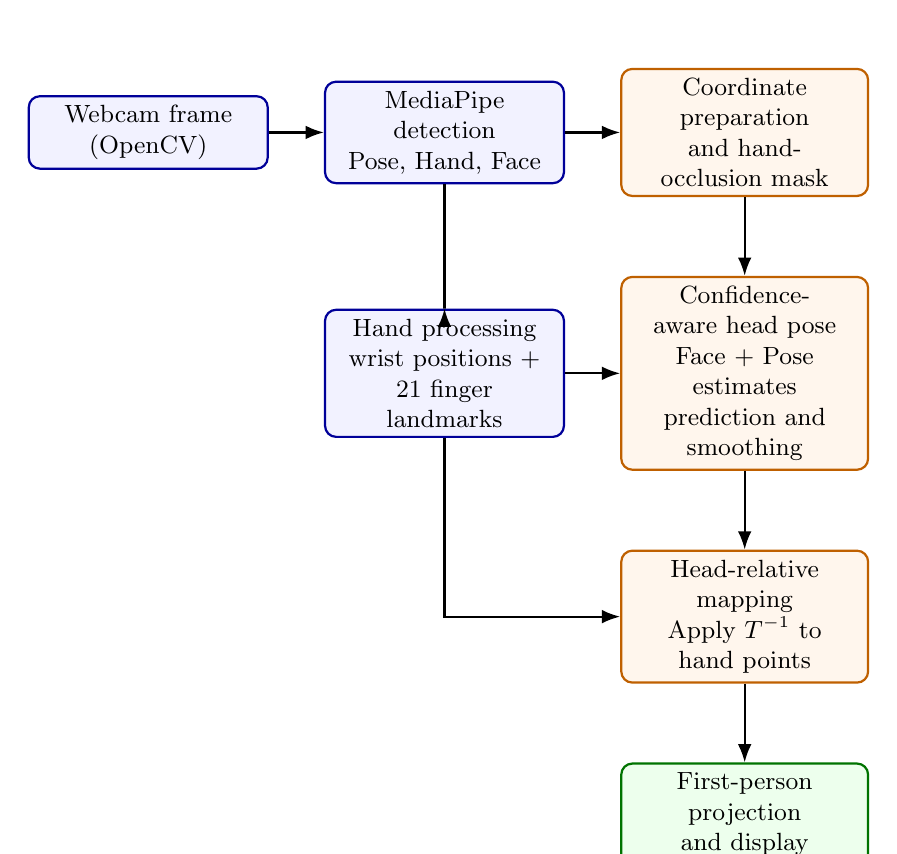
\begin{tikzpicture}[>=Latex,node distance=0.55cm and 0.7cm,
        stage/.style={draw=blue!60!black,fill=blue!5,rounded corners,thick,align=center,text width=2.8cm,minimum height=0.85cm,font=\small},
        process/.style={draw=orange!75!black,fill=orange!7,rounded corners,thick,align=center,text width=2.9cm,minimum height=0.95cm,font=\small},
        output/.style={draw=green!45!black,fill=green!7,rounded corners,thick,align=center,text width=2.9cm,minimum height=0.85cm,font=\small},
        arrow/.style={->,thick}]
        \node[stage] (capture) {Webcam frame\\(OpenCV)};
        \node[stage,right=of capture] (detect) {MediaPipe detection\\Pose, Hand, Face};
        \node[process,right=of detect] (prep) {Coordinate preparation\\and hand-occlusion mask};
        \node[process,below=1cm of prep] (head) {Confidence-aware head pose\\Face + Pose estimates\\prediction and smoothing};
        \node[stage,left=of head] (hands) {Hand processing\\wrist positions +\\21 finger landmarks};
        \node[process,below=1cm of head] (transform) {Head-relative mapping\\Apply $T^{-1}$ to hand points};
        \node[output,below=1cm of transform] (render) {First-person projection\\and display};
        \draw[arrow] (capture)--(detect);
        \draw[arrow] (detect)--(prep);
        \draw[arrow] (prep)--(head);
        \draw[arrow] (detect.south) |- (hands.north);
        \draw[arrow] (hands)--(head);
        \draw[arrow] (head)--(transform);
        \draw[arrow] (hands.south) |- (transform.west);
        \draw[arrow] (transform)--(render);
    \end{tikzpicture}
    \caption{Processing pipeline of the prototype, from webcam acquisition and MediaPipe landmark detection to head-relative hand mapping and first-person display.}
    \label{fig:pipeline}
\end{figure}


\subsection{Head-Pose Estimation}

The head-pose estimator is important because the head coordinate frame determines how the tracked hands appear in the first-person view. If the estimated head orientation changes incorrectly, the mapped hand positions may also appear to shift.

The prototype uses two sources of head-orientation information:

\begin{itemize}
    \item \textbf{Face Landmarker.} The rotation component of the facial transformation matrix provides an estimate of face orientation. The prototype reduces its confidence when selected facial landmarks are estimated to be covered by a hand.
    \item \textbf{Pose Landmarker.} The nose, eyes, and ears provide a second estimate. A weighted rigid alignment fits a predefined head model to the detected 3D landmarks. The estimate receives less confidence when too few landmarks are reliable or when the fit residual is large.
\end{itemize}

The two orientation estimates are combined using confidence-weighted spherical interpolation. If their orientations disagree substantially, the estimator gives priority to the more trusted estimate.

The prototype also predicts the head's next orientation and position using its estimated angular and linear velocities. Measurements that differ greatly from the prediction are down-weighted rather than immediately rejected. Adaptive smoothing reduces jitter when the head is relatively still while allowing faster response during head turns. When measurements become unreliable, the estimator temporarily continues from its prediction and gradually incorporates measurements again when confidence improves.

\begin{figure}[h!]
    \centering
    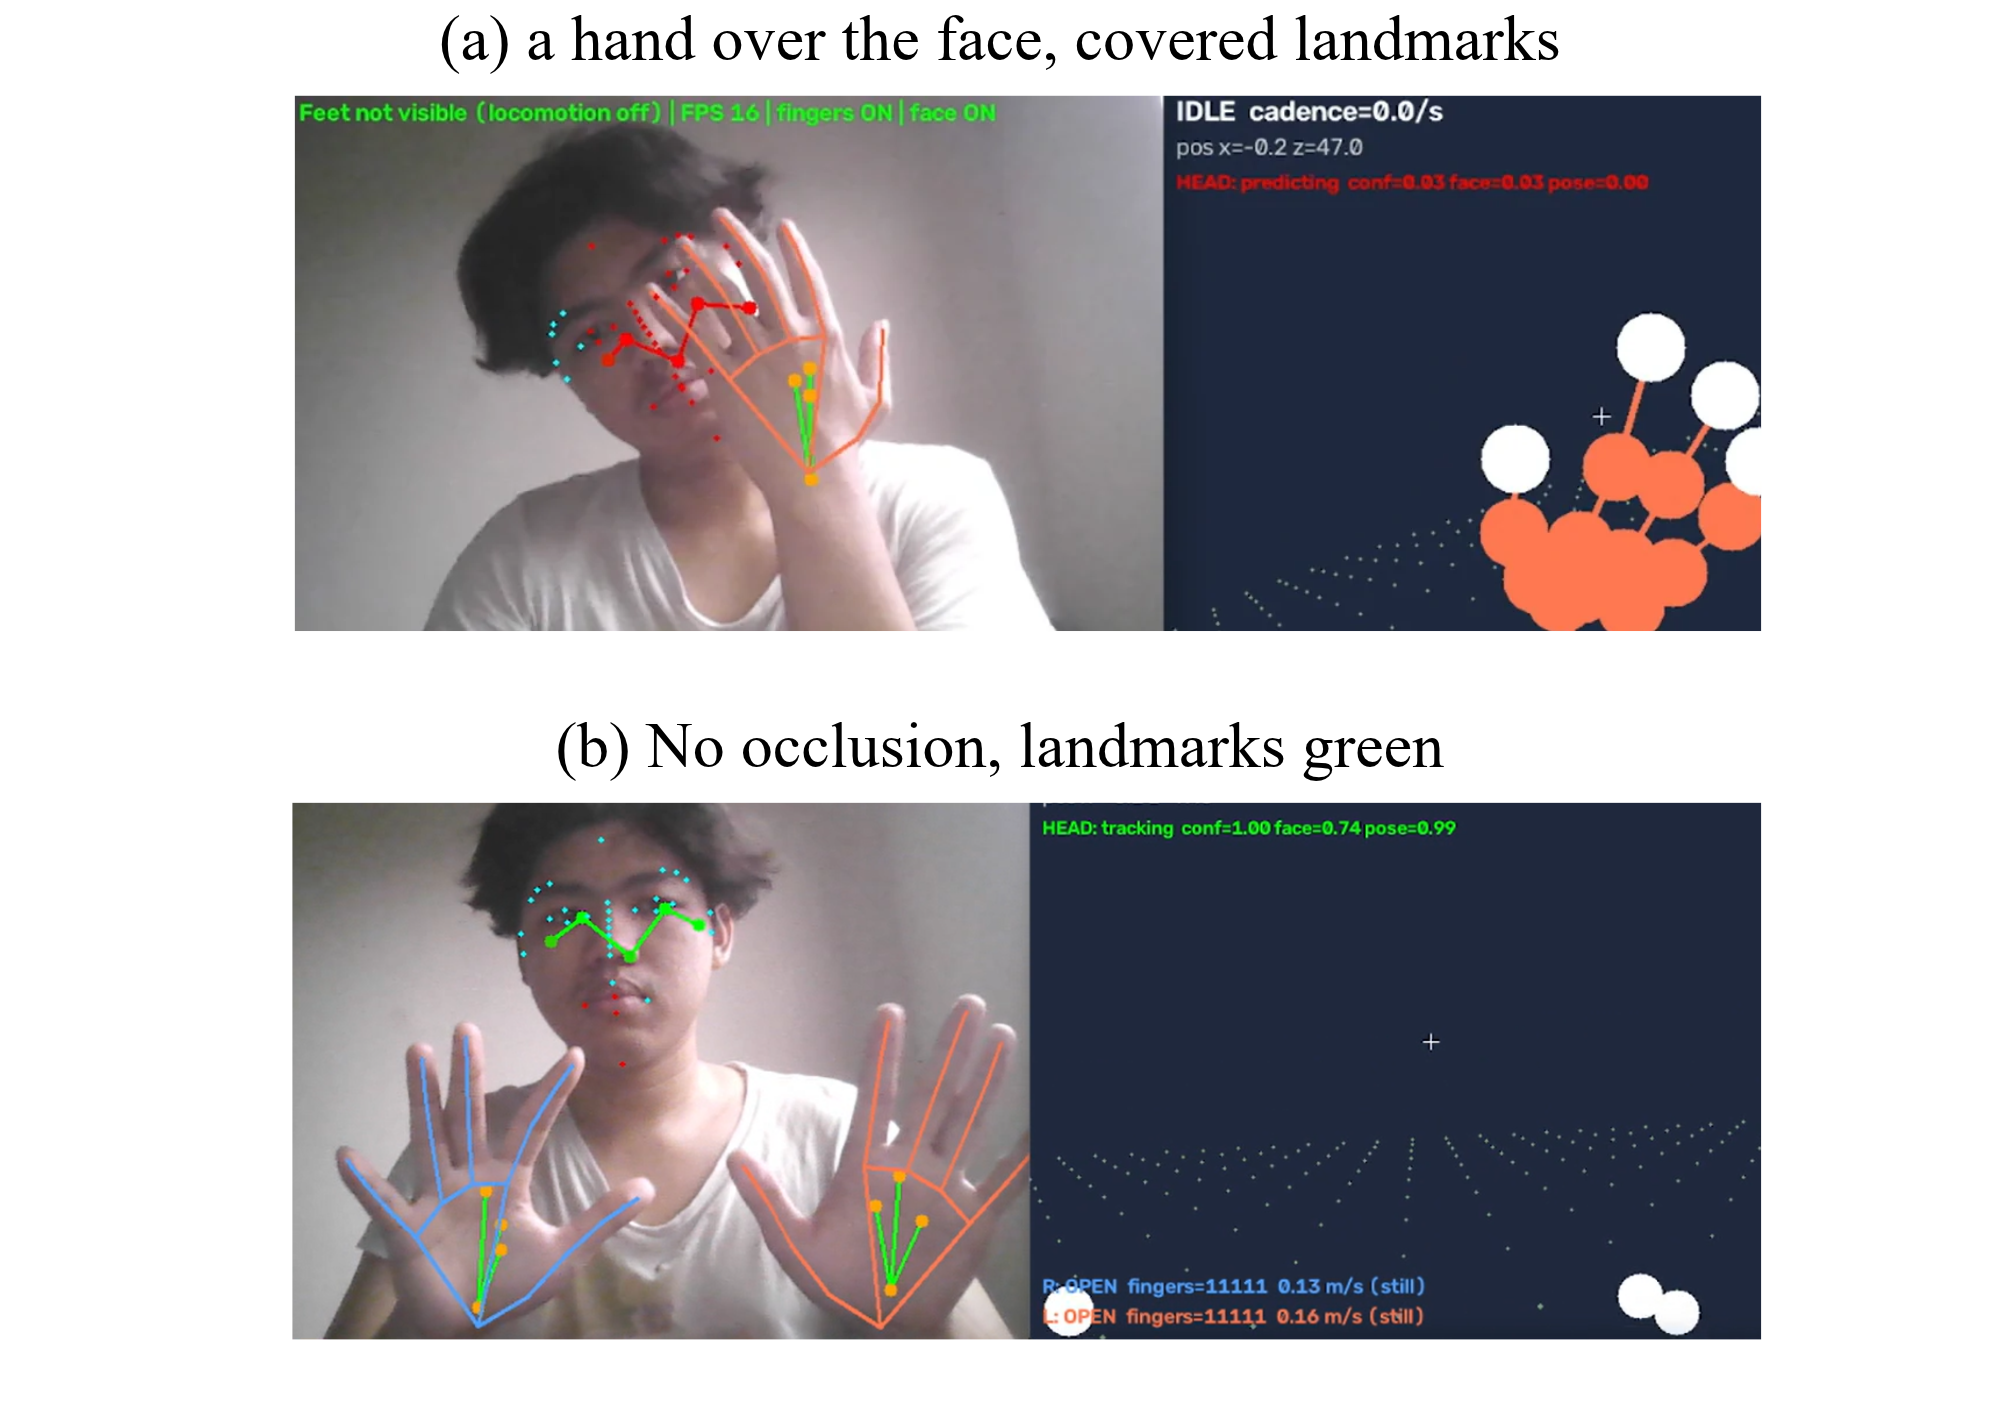
\includegraphics[width=0.9\linewidth]{assets/Figure3.png}
    \caption{Prototype webcam view showing the detected head landmarks and confidence indicators.}
    \label{fig:headtracking}
\end{figure}

\subsection{Hand and Finger Mapping}

The Pose Landmarker provides wrist positions, which are used to establish the global position of each hand relative to the head. The Hand Landmarker provides 21 landmarks for each detected hand, describing the palm and finger configuration.

The prototype pairs each detected hand with a pose wrist using their image-space proximity. It then expresses the finger landmarks as offsets from the hand wrist. These offsets are combined with the wrist position obtained from the Pose Landmarker. This allows the system to retain the hand's position relative to the body while representing the detailed shape of the fingers.

The combined hand points are transformed using $T^{-1}$ and projected onto the first-person display. The prototype also applies distance-based rules to estimate finger extension and classify simple hand configurations, including OPEN, FIST, POINT, PEACE, THUMB, and PINCH.


\begin{figure}[h!]
    \centering
    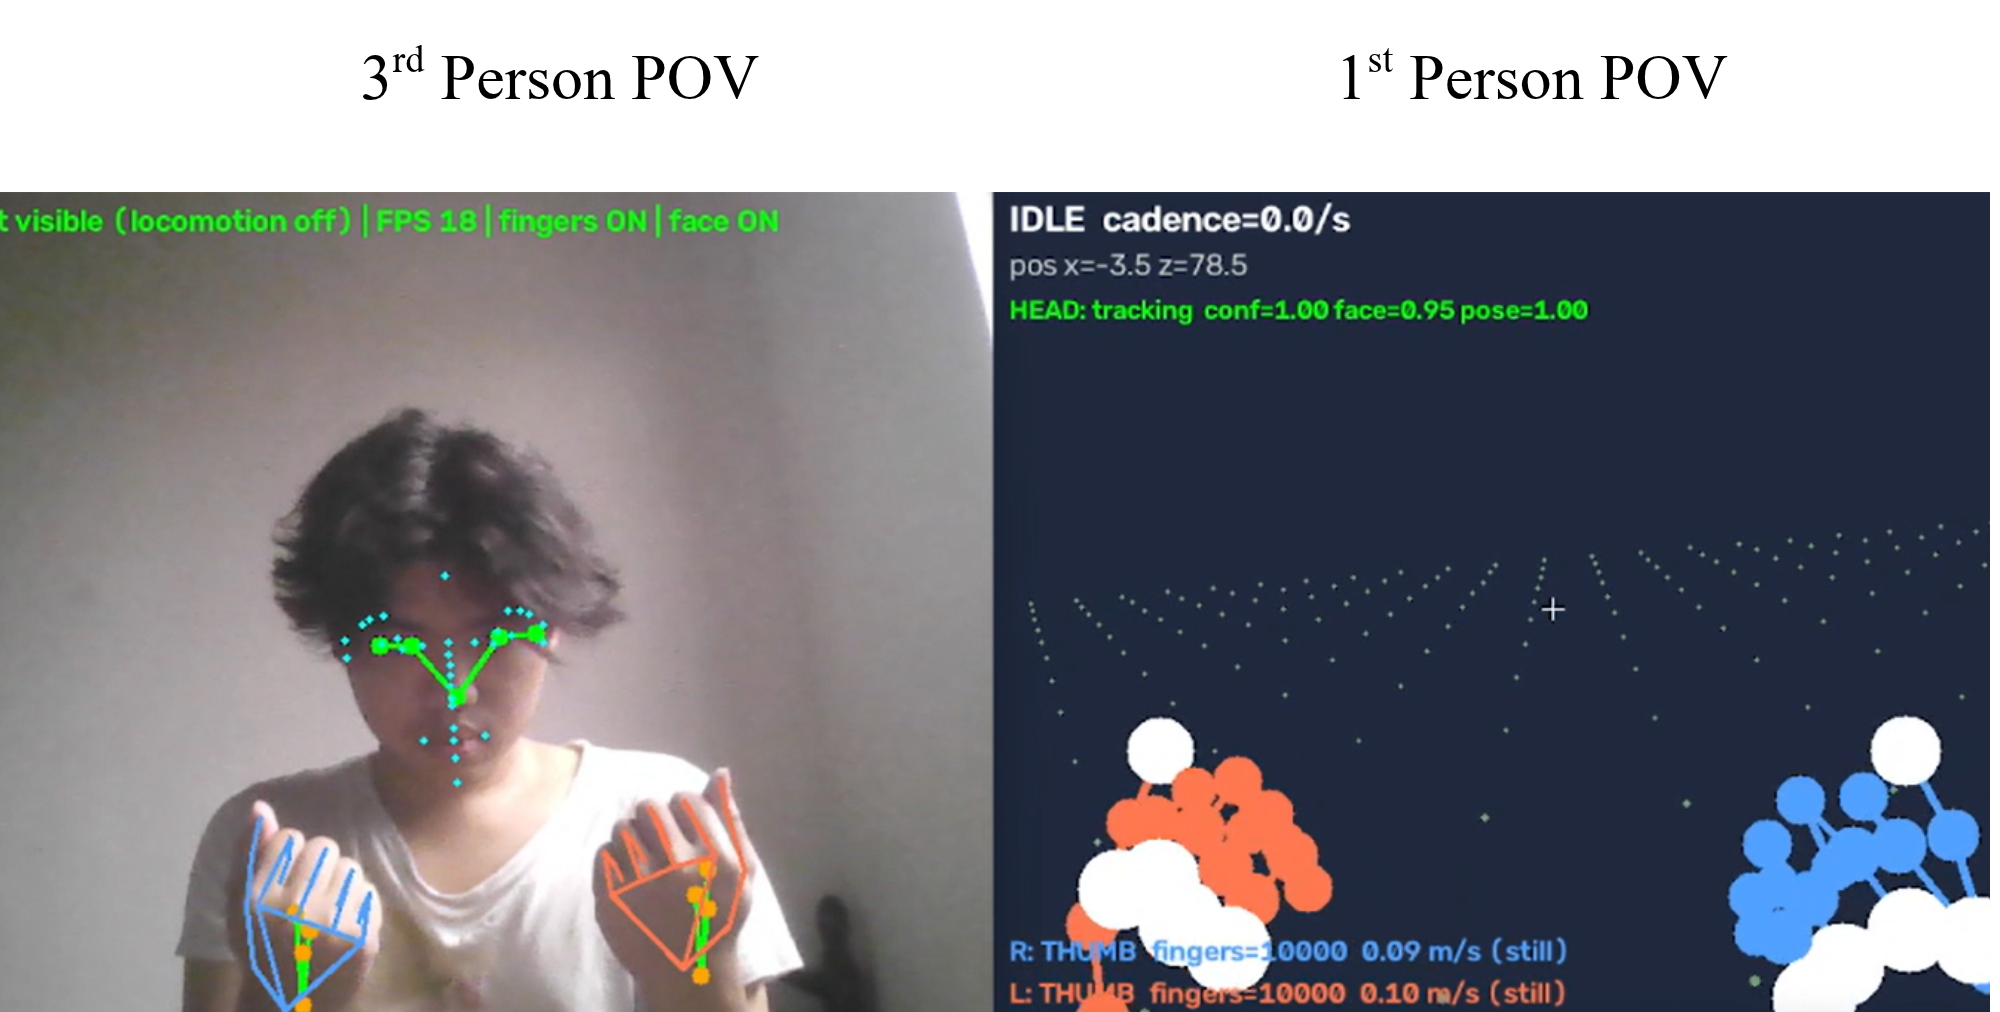
\includegraphics[width=0.9\linewidth]{assets/Figure4.png}
    \caption{Third-person webcam view and corresponding first-person hand representation.}
    \label{fig:3rdand1stpersonView}
\end{figure}

\subsection{Implementation Details}

The prototype is implemented in Python and uses the MediaPipe Tasks API. The source file initializes three MediaPipe tasks: Pose Landmarker, Hand Landmarker, and Face Landmarker. The Hand and Face Landmarker model files are downloaded automatically by the script if they are not already present in the project directory. The Pose Landmarker model file must be available beside the script.

\begin{table}[h!]
    \centering
    \caption{Prototype implementation details}
    \label{tab:implementation}
    \small
    \begin{tabular}{>{\raggedright\arraybackslash}p{5cm} >{\raggedright\arraybackslash}p{8cm}}
        \toprule
        Item & Implementation \\
        \midrule
        Programming language      & Python \\
        Pose estimation           & MediaPipe Pose Landmarker \\
        Hand tracking             & MediaPipe Hand Landmarker \\
        Face tracking             & MediaPipe Face Landmarker \\
        Image capture and display & OpenCV \\
        Numerical operations      & NumPy \\
        Pose model file           & \texttt{pose\_landmarker\_full.task} \\
        Hand and face model files & \texttt{hand\_landmarker.task}, \texttt{face\_landmarker.task} \\
                                  & (downloaded automatically by the script when absent) \\
        First-person display size & $640 \times 480$ pixels \\
        \bottomrule
    \end{tabular}
\end{table}


\subsection{Evaluation and Data Collection}

\begin{enumerate}[label=(\alph*)]
    \item \textbf{Detection continuity:} whether the head, wrists, and fingers remain detected during each test scenario.
    \item \textbf{View stability:} whether the first-person display remains visually stable when the user's head is still.
    \item \textbf{Occlusion response:} how the head-pose estimate behaves when a hand covers part of the face.
    \item \textbf{Recovery behavior:} whether the estimate returns smoothly after the face becomes visible again.
    \item \textbf{Processing speed:} the frames per second displayed by the running prototype.
    \item \textbf{Gesture output:} whether the displayed hand configuration agrees with the hand configuration performed.
\end{enumerate}

\begin{table}[h!]
    \centering
    \caption{Test environment}
    \label{tab:setup}
    \small
    \begin{tabular}{>{\raggedright\arraybackslash}p{4cm} >{\raggedright\arraybackslash}p{9cm}}
        \toprule
        Item & Value \\
        \midrule
        Processor & Processor	13th Gen Intel(R) Core(TM) i5-13450HX, 2400 Mhz, 10 Core(s), 16 Logical Processor(s) \\
        System memory & 8 GB RAM \\
        Graphics processor & NVIDIA GeForce RTX 3050 8gb \\
        Webcam model and resolution & FHD 1080p\\
        Camera distance & 1.5 m (assumed distance for framing the head and upper torso) \\
        Lighting condition & Ideal, evenly distributed frontal lighting with minimal shadows and no strong backlighting \\
        MediaPipe version & To be recorded from the installed environment \\
        Python version & To be recorded from the installed environment \\
        Number of participants & 1 (assumed participant height: 165 cm) \\
        \bottomrule
    \end{tabular}
\end{table}

\section{Main Discussion, Results, and Analysis}

\subsection{Illustrative Scenarios}

Table~\ref{tab:scenarios} describes scenarios that can be used to inspect the behavior of the prototype. The expected behavior follows from the design of the processing pipeline. The observed behavior must be completed using actual tests and screenshots; it is not inferred from the source code alone.

\begin{table}[h!]
    \centering
    \caption{Illustrative test scenarios}
    \label{tab:scenarios}
    \small
    \begin{tabular}{>{\raggedright\arraybackslash}p{3.0cm} >{\raggedright\arraybackslash}p{5.3cm} >{\raggedright\arraybackslash}p{6.1cm}}
        \toprule
        Scenario & Expected behavior & Preliminary observation from implementation \\
        \midrule
        Both hands visible & The system detects the wrists and finger landmarks and displays the mapped hands in the first-person window. & Pose Landmarker succesfully supplied wrist positions, while Hand Landmarker supplied detailed finger positions. The two sources are combined and were able to display the hand geometry on a first person perspective.\\
        Head turned while hands remain visible & The head coordinate frame changes orientation, and the mapped hand positions are re-expressed relative to that frame. & The movement was accurately interpreted on a first person perspective, eliminating the hand when the head should not realistically see it.\\
        One hand covers part of the face & The affected head landmarks receive reduced confidence, and the estimator relies more on other measurements and its prediction. & The hand mask reduces the weights of covered facial and pose landmarks. The estimator can continue using remaining measurements and temporal prediction, but it causes inaccuracy such as excessive tilting of the perspective.\\
        Hand moves across the face & The head-pose estimate should avoid abrupt changes and should incorporate reliable measurements again after the face becomes visible. & Confidence is reduced as the hand mask covers facial landmarks. Prediction and adaptive smoothing are intended to limit abrupt changes and ease the estimate back toward new measurements. \\
        Hand configuration changes & The detected finger landmarks are used to classify the corresponding hand configuration when the hand is sufficiently visible. & The prototype evaluates finger extension and pinch distance to classify configurations such as OPEN, FIST, HAND FACING AWAY, POINT, PEACE, THUMB, and PINCH.\\
        \bottomrule
        \end{tabular}
\end{table}

\begin{table}[h!]
    \centering
    \caption{Qualitative observations of the prototype}
    \label{tab:observations}
    \small
    \begin{tabular}{>{\raggedright\arraybackslash}p{4cm} >{\raggedright\arraybackslash}p{9cm}}
        \toprule
        Test condition & Preliminary qualitative observation based on the implemented prototype \\
        \midrule
        Head facing the webcam & The Face and Pose Landmarkers provide the measurements used to initialize the head coordinate frame. The first-person display becomes available after the estimator obtains a sufficiently confident initial estimate, it managed to track the 3rd person pov head movements and was successful in mapping them to first person perspective, responding to head yaws accurately\\
        Head turning left and right & Changes in the estimated head orientation update the head-relative coordinate frame. Consequently, mapped hand positions are re-expressed relative to the updated viewpoint. \\
        Hand landmarks visible & Pose wrist landmarks establish hand position, while the Hand Landmarker supplies finger configuration. When paired successfully, the prototype displays the combined hand geometry in the first-person window. \\
        Hand partially covering the face & The hand-occlusion mask lowers the confidence assigned to covered facial and pose landmarks. However the system still struggles estimating head position whenever it is obscured by the hand, causing inaccurate tilting on the 1st person perspective. \\
        Hand moving across the face & The estimator is designed to reduce the influence of covered facial landmarks and use temporal prediction and adaptive smoothing. The implementation aims to avoid sudden changes and resume measurement-based tracking as confidence returns.
        As a result there were no inconsistent movements whenever the hand moves across the face but it varies by how long it remains obscured\\
        Finger configuration changes & The prototype evaluates finger extension and thumb-index distance to classify selected configurations, including OPEN, FIST, HANDS FACING FRONT, HANDS FACING BACK, THUMB, and PINCH \\
        \bottomrule
        \end{tabular}
\end{table}

\subsection{Discussion and Limitations}

The prototype demonstrates how webcam-derived landmarks can be expressed in a different coordinate frame through a homogeneous matrix transformation. The head-pose estimate supplies the transformation, while the wrist and finger landmarks provide the hand geometry to be mapped. The implementation also combines multiple landmark sources and confidence-aware processing to reduce the effect of facial occlusion.

The following limitations should be considered when interpreting the prototype:

\begin{itemize}
    \item \textbf{Depth ambiguity.} A single webcam estimates depth from visual information, so the $z$ coordinate may be less reliable than image-plane coordinates.
    \item \textbf{Occlusion.} If a hand or another object obscures the face or hands, the corresponding landmarks may become unreliable or disappear.
    \item \textbf{Occlusion-mask dependence.} The hand-based occlusion estimate depends on the hand being detected. If the hand is not detected, the mask may fail to identify the covered facial region.
    \item \textbf{No eye-gaze tracking.} The system estimates head orientation, not the user's exact gaze direction. Eye movement independent of head movement is not represented.
    \item \textbf{Rule-based gesture classification.} Finger configurations are classified using fixed distance rules. Unusual hand poses or tracking errors may lead to incorrect classifications.
    \item \textbf{Geometric representation.} The first-person window is a geometric visualization of mapped hands and fingers, not a reconstructed photographic view of the user's \mbox{surroundings}.
    \item \textbf{Processing requirements.} Running pose, hand, and face models in the same frame requires more computation than running a single model. The actual frame rate depends on the computer, camera input, and runtime configuration.
    \item \textbf{No external application integration.} The current prototype displays the mapped output in its own window. Integration with a game engine or VR application has not been established by the provided implementation.
\end{itemize}

\section{Conclusion}

This paper presented a webcam-based prototype for mapping third-person hand landmarks into a first-person coordinate representation. MediaPipe Pose, Hand, and Face Landmarkers provide the estimated landmarks and facial transformation data. A homogeneous transformation matrix defines the relationship between the third-person coordinate frame and the head-relative first-person frame, allowing wrist and finger positions to be re-expressed relative to the estimated eye position and orientation.

The prototype also incorporates confidence-aware head-pose estimation. It considers landmark visibility and hand occlusion, combines orientation estimates from the Face and Pose Landmarkers, and uses prediction and adaptive smoothing to reduce abrupt changes when facial landmarks become unreliable. The implementation demonstrates the integration of AI-based landmark estimation with coordinate geometry and matrix operations. Quantitative claims about accuracy, stability, and processing performance should only be made after completing the proposed tests and recording their results.

\section{Recommendations and Future Directions}

\begin{itemize}
    \item
    \textbf{Movement Tracking via ankle/feet tracker.} An earlier version of the prototype included ankle-based walk and run detection to move the first-person viewpoint, but it was removed because locomotion tracking falls outside the scope of this study, which focuses on mapping head-relative hand and finger positions. This however can be added in re-added in future iterations to explore movement, particularly in VR applications.
    
    \item \textbf{Quantitative evaluation.} Conduct repeated trials under different lighting conditions, camera distances, head orientations, and hand-occlusion scenarios. Record frame rate, detection continuity, and head-view stability.
    \item \textbf{Improved depth estimation.} Investigate calibration methods or additional camera input to reduce uncertainty in estimated depth coordinates.
    \item \textbf{Personalized calibration.} Adapt the head model to individual facial proportions during an initial calibration procedure.
    \item \textbf{Gesture recognition.} Evaluate the current distance-based gesture rules and consider a trained classifier if a sufficiently varied hand-pose dataset becomes available.
    \item \textbf{Eye tracking.} Investigate whether gaze estimation can be incorporated so that the first-person representation accounts for eye movement independently of head orientation.
    \item \textbf{Application integration.} Explore sending the calculated head and hand transformations to a game engine or VR application. This should be treated as future work until implemented and evaluated.
\end{itemize}

\newpage
\begin{thebibliography}{99}

\bibitem{blazepose}
Bazarevsky, V., Grishchenko, I., Raveendran, K., Zhu, T., Zhang, F., \& Grundmann, M. (2020).
BlazePose: On-device real-time body pose tracking.
\textit{arXiv preprint arXiv:2006.10204}.
\url{https://arxiv.org/abs/2006.10204}

\bibitem{kim2016}
Kim Y, Park H, Bang S, \&Lee SH. Retargeting Human-Object Interaction to Virtual Avatars.
\textit{Kim Y, Park H, Bang S, Lee SH. Retargeting Human-Object Interaction to Virtual Avatars. IEEE Trans Vis Comput Graph. 2016 Nov;22(11):2405-12. doi: 10.1109/TVCG.2016.2593780. Epub 2016 Jul 27. PMID: 27479972.}
\url{https://pubmed.ncbi.nlm.nih.gov/27479972/}

\bibitem{rgbavatar}
Poulios, I., Pistola, T., Symeonidis, S., Diplaris, S., Ioannidis, K., Vrochidis, S., \& Kompatsiaris, I. (2024).
Enhanced real-time motion transfer to 3D avatars using RGB-based human 3D pose estimation.
In \textit{Proceedings of the ACM International Conference on Interactive Media Experiences (IMX 2024)}.
\url{https://doi.org/10.1145/3672406.3672427}

\bibitem{telerehab}
Clemente, C., Chambel, G., Silva, D. C. F., Mesquita Montes, A., Pinto, J. F., \& Pl\'acido da Silva, H. (2024).
Feasibility of 3D body tracking from monocular 2D video feeds in musculoskeletal telerehabilitation.
\textit{Sensors, 24}(1), 206.
\url{https://doi.org/10.3390/s24010206}

\bibitem{yiannakides2019}
Yiannakides, A. (2019).
Real-time 3D human pose and motion reconstruction from monocular RGB videos.
\textit{Computer Animation and Virtual Worlds, 30}(3--4), e1887.
\url{https://doi.org/10.1002/cav.1887}

\bibitem{mediapipe}
Google. (n.d.). \textit{MediaPipe Solutions: Pose Landmarker, Hand Landmarker, and Face Landmarker}.
Google AI Edge.
\url{https://developers.google.com/edge/mediapipe/solutions/guide}

\end{thebibliography}

\newpage
\appendix
\section{How to Run the Prototype}

\begin{enumerate}[label=\arabic*.]
    \item \textbf{Extract the program.} Right-click \texttt{program.zip}, choose \textit{Extract All}, and open the extracted folder.
    \item \textbf{Install the requirements.} Install Python if it is not yet installed. Then open a command prompt inside the extracted folder (type \texttt{cmd} in the folder's address bar and press Enter) and run:
    \cmdline{pip install -r requirements.txt}
    This installs the required packages: MediaPipe, OpenCV, and NumPy.
    \item \textbf{Check the model file.} Make sure the\texttt{.task} files are in the same folder\\ as \texttt{Implementation.py}.
    \item \textbf{Run the program.} Connect a webcam and double-click the \texttt{run.bat} file in the extracted folder. On the first run, the script downloads the Hand and Face Landmarker model files automatically if they are not already present.
    \item \textbf{Use the controls.} Press \texttt{q} to quit, \texttt{h} to toggle finger tracking, and \texttt{f} to toggle the Face Landmarker.
\end{enumerate}

\section{Prototype Screenshots}


\begin{figure}[h!]
    \centering
    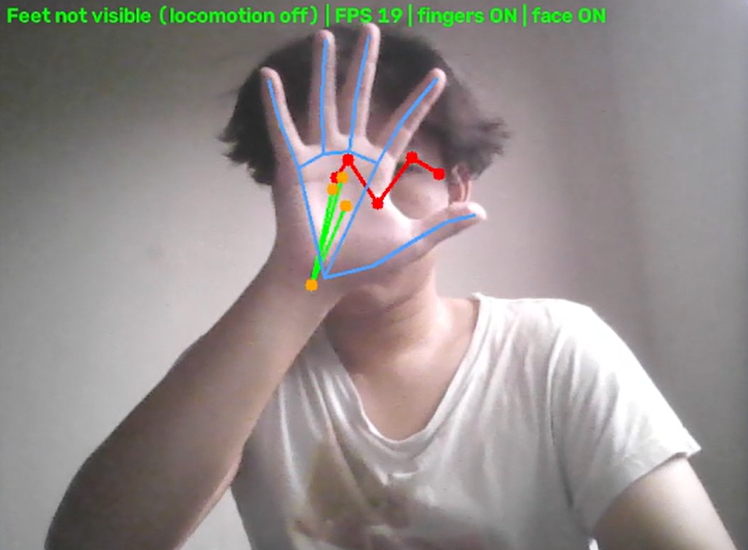
\includegraphics[width=0.9\linewidth]{assets/Figure5.png}
    \caption{Prototype webcam view showing the detected head landmarks and confidence indicators.}
    \label{fig:ThirdPerson}
\end{figure}

\begin{figure}[h!]
    \centering
    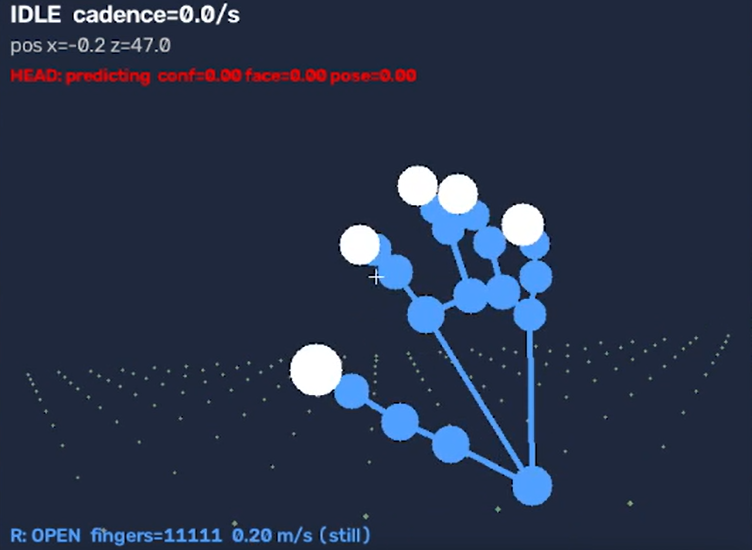
\includegraphics[width=0.9\linewidth]{assets/Figure6.png}
    \caption{First-person window showing the mapped hand and finger representation.}
    \label{fig:FirstPerson}
\end{figure}

\end{document}
